A deflexão lateral produzida por uma carga sobre um pilar compõe o processo conhecido como \textbf{flambagem por flexão}. Ela ocorrerá sempre em torno do eixo de menor momento de inércia de sua seção transversal, pois gerará o maior índice de esbeltez.

Para calcular o índice de esbeltez é necessário o comprimento de flambagem, que é dado de acordo com o tipo de vinculação na base e no topo do pilar.

\begin{figure}[H]
	\begin{center}
	\caption{Comprimento de flambagem para diferentes pilares.}
    	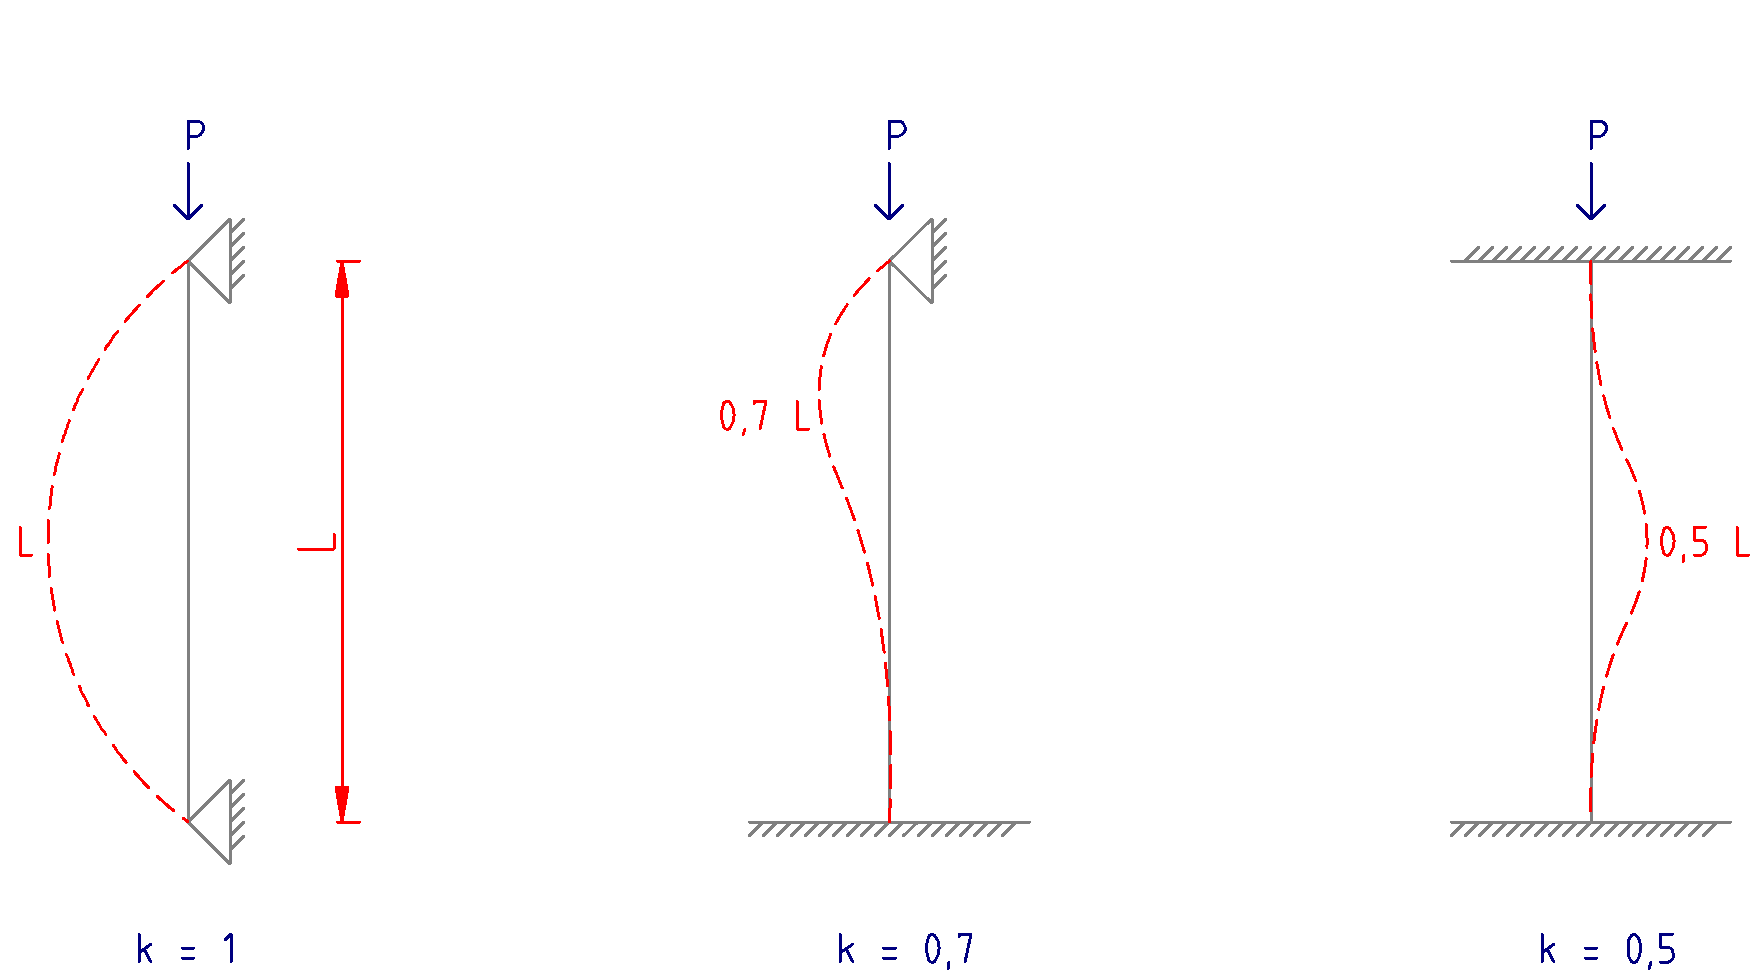
\includegraphics[width=\textwidth]{Comprimento-de-flambagem/Imagens/Comprimento-de-flambagem-0.png}
	\end{center}
\end{figure}

Porém, a NBR 6118, item 15.8.2 diz: Caso seja pilar engastado e livre no topo, o valor de $L_e=2\cdot L$. Nos demais casos, adotar o comprimento equivalente calculado anteriormente pela Equação~\eqref{equacao-comprimento-equivalente}.

\begin{figure}[H]
	\begin{center}
	\caption{Comprimento de flambagem de um pilar engastado na base e livre no topo.}
    	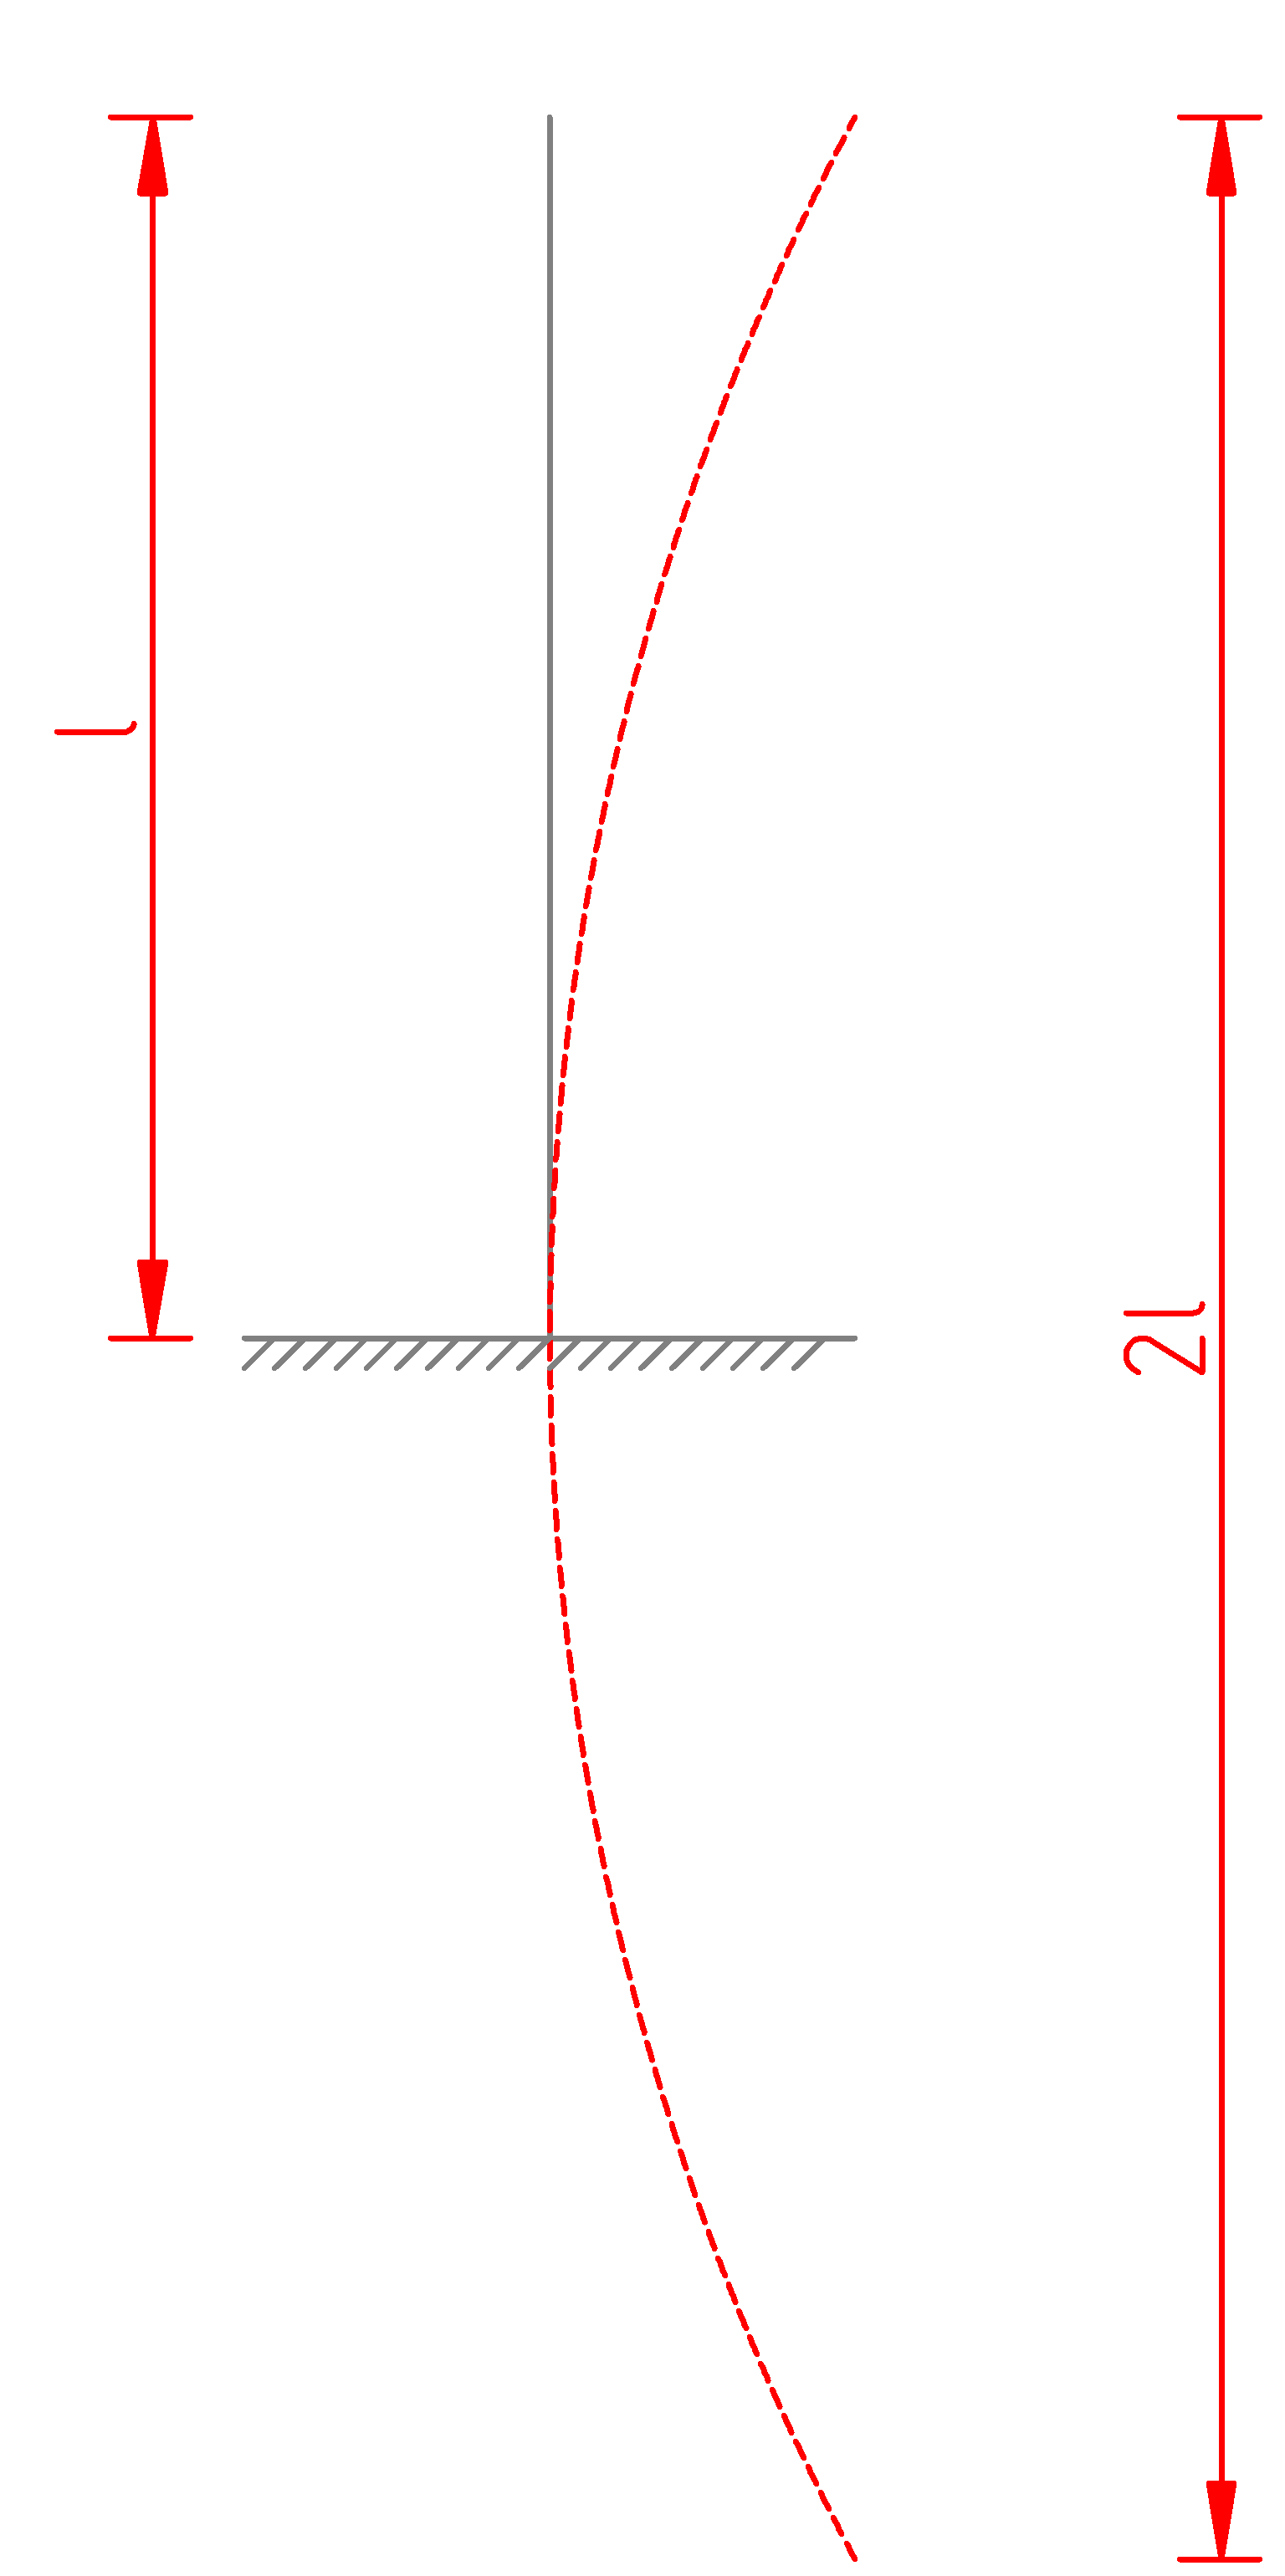
\includegraphics[width=0.3\textwidth]{Comprimento-de-flambagem/Imagens/Comprimento-de-flambagem-1.png}
	\end{center}
\end{figure}